% use lualatex to compile, for some reason xelatex fails for the {Libertinus Serif} font.
\documentclass[11pt]{book}
%\documentclass[11pt]{amsart} % fails on title, date, etc.

% ---------- Fonts (LuaLaTeX / XeLaTeX) ----------
\usepackage{fontspec}
\setmainfont{Libertinus Serif}
%\setmainfont{TeX Gyre Pagella}
%\setsansfont{TeX Gyre Heros}
\setmonofont{Inconsolata}

% ---------- Page layout ----------
\usepackage[a4paper,margin=1.1in]{geometry}

% ---------- Math & theorem setup ----------
\usepackage{amsmath,amssymb,amsthm,mathtools}

\theoremstyle{definition}
\newtheorem{definition}{Definition}

\theoremstyle{plain}
%\newtheorem{theorem}[definition]{Theorem}
\newtheorem{theorem}{Theorem}
\newtheorem{lemma}{Lemma}
\newtheorem{proposition}{Proposition}
\newtheorem{corollary}{Corollary}
\newtheorem{exercise}{Exercise}[chapter]



\usepackage{xcolor}
\newtheoremstyle{problemstyle} % name
  {3pt} % Space above
  {3pt} % Space below
  {\normalfont} % Body font
  {} % Indent
  {\bfseries\color{blue}} % Theorem head font
  {.} % Punctuation
  { } % Space after head
  {} % Head spec
\theoremstyle{problemstyle}
\newtheorem{problem}{Problem}


\theoremstyle{remark}
\newtheorem*{remark}{Remark}
\renewcommand\qedsymbol{$\blacksquare$}
% the reflection box
\usepackage[framemethod=tikz]{mdframed}
\theoremstyle{definition}
\newtheorem{reflection}{Reflection}
\mdfdefinestyle{reflectionbox}{
  innertopmargin=\topskip,
  roundcorner=5pt,
  linecolor=cyan,
  backgroundcolor=cyan!20,
}
\surroundwithmdframed[style=reflectionbox]{reflection}
% the reflection box
% quotes
\usepackage[style=english]{csquotes}
\MakeOuterQuote{"}
% quotes

% epigraphs
% I chose epigraph-keys for its simplicity
\usepackage{epigraph-keys}
% epigraphs

%images
\usepackage{graphicx}
\usepackage{float}
\usetikzlibrary{graphs,graphdrawing,intersections,calc,patterns}
\usegdlibrary{trees}
%images
% ---------- Typography ----------
\usepackage{microtype}

%plots
\usepackage{pgfplots}
%plots

% multiple columns
\usepackage{multicol}
\setlength{\columnseprule}{1pt}
\def\columnseprulecolor{\color{blue}}
% multiple columns
%multirow (tables) using makecell
\usepackage{makecell}
\renewcommand\theadfont{\bfseries}
%multirow (tables) using makecell

%canceling terms
\usepackage{cancel}
%canceling terms

%customize lists
\usepackage{enumitem}
%customize lists

% comment out large portions, but document them in source 
\usepackage{comment}
% comment out large portions, but document them in source 

% bib
\usepackage[
  backend=biber,
  style=numeric
]{biblatex}

\addbibresource{refs.bib}
% bib

%macros
\DeclareMathOperator{\size}{size}
\newcommand{\sizex}{\size(\boldsymbol{x})}
\newcommand{\sizea}{\size(\boldsymbol{a})}
\newcommand{\sizeb}{\size(\boldsymbol{b})}
\newcommand{\sizec}{\size(\boldsymbol{c})}
\newcommand{\sized}{\size(\boldsymbol{d})}
\DeclareMathOperator{\nnz}{nnz} % number of nonzero elements in a (sparse) vector
\newcommand{\nnzx}{\nnz(\boldsymbol{x})}
%macros
% https://github.com/plk/biber/issues/373
\DeclareBibliographyAlias{movie}{misc}
% https://github.com/plk/biber/issues/373
% ---------- Hyperlinks ----------
\usepackage[hidelinks]{hyperref}

% ---------- Metadata ----------
\title{Notes on \\ \emph{Applied Linear Algebra}
\\ \emph{by Stephen Boyd and Lieven Vandenberghe}
\\ \emph{(Vectors, Matrices, and Least Squares)}}
\author{Kedar Mhaswade}
\date{29 May 2026}

\begin{document}
\maketitle
\begin{reflection}[Introduction]
    These are the author's highly personal notes based on this book \cite{bv-app-lin-alg}. They may occasionally sound like author's conversation with the reader (or even himself). Even if they are personal and appear in the public domain, they may help the reader, although the author isn't exactly sure how. He wrote them for 0) the love of mathematics and writing 1) \LaTeX{} practice (of writing hopefully readable mathematics, albeit longer than appearing in standard texts), and 2) reliable archival (paper, on which most math is created, tends to get lost) that incurs minimal overhead.

    These notes are interspersed with ``reflection boxes'' like this one. They are meant to express author's `rough' thinking process (mental catharsis of sorts), of which frustration is often an inseparable part. The author writes mostly in first person for an authentic conversational tone.

\end{reflection}

\section{Preface}

\epigraph[author={Paul Halmos}, source={I Want to be a Mathematician \cite{halmos-iwtbam}}, width={0.7\textwidth}]
{
    Audience, level, and treatment--a description of such matters is what prefaces are supposed to be about.
}

This book says the following (emphasis mine):
\epigraph[author={Boyd and Vandenberghe}, source={Applied Linear Algebra \cite{bv-app-lin-alg}}, width={0.7\textwidth}]
{
    Our goal is to give the beginning student, with little or no prior exposure to linear algebra, \textbf{a good grounding in the basic ideas, as well as an appreciation for how they are used in many applications, including data fitting, machine learning and artificial intelligence}, tomography ((medicine) obtaining pictures of the interior of the body), navigation, image processing, finance, and automatic control systems.
}

The book is an introductory linear algebra text for undergrad students, with an emphasis on applications. A cursory glance suggests that the book takes a more algebraic approach (and uses geometric intuition sparingly).

I believe that is the right level for my first reading. It further says:

\epigraph[author={Boyd and Vandenberghe}, source={Applied Linear Algebra \cite{bv-app-lin-alg}}, width={0.7\textwidth}]
{
    If you read the whole book, \textbf{work some of the exercises}, and carry out computer exercises to implement or use the ideas and methods, you will learn a lot.
}

This document contains my notes on the material in this book and my answers to exercises. These notes follow the book's structure.


\chapter{Vectors}

\section{Vectors}
\begin{reflection}
    This section has several definitions, some of them are subtle. Since I believe that this book prefers an algebraic formalism more than geometric intuition, definitions are key to its treatment and to my understanding, however formal. Formalism doesn't imply a lack of creativity, but it aligns well with the abstract nature of mathematics: You make up certain (abstract) objects and operations on them (define them), let them interact with each other (again, no concrete operations are intended), and see if a structure emerges.

    Is this abstract, algebraic ``definitions, theorems, proofs, synthetic exercises and problems, and practical examples'' approach more `dry' than a more visual, geometric, or physical approach where vectors start out their lives as directed line segments in space? Perhaps it is. There's always a tension between these two fundamental (algebraic, geometric) approaches. One has got to figure out what one comes to like. 

    \epigraph[author=Jürgen Jost, source=Mathematical Concepts \cite{jost-mc}]{
        Mathematics translates concepts into formalisms and applies those formalisms to derive insights that are usually not amenable to a less formal analysis.
    }

    One `strength' of the algebraic approach may be in avoiding a head-on collision with the ``curse of dimesionality'' (a term that, I think, was first introduced by the mathematician Richard Bellman \cite{curse-of-dimensionality}) which concerns the puzzling properties of a higher dimensional Euclidean space. Since the visualization of an $n$-dimensional space is hard for us when $n\ge 4$, abandoning the geometric interpretation may aid understanding. This is because in this approach, we do \emph{not} treat a $2-$ or $3-$dimensional space as something special or different.

    I have tried another book that appeals to properties of a `physical' space, Banesh Hoffmann's \emph{About Vectors} \cite{hoffmann-av}, and I have found it useful, but to complement that approach, I will follow a more abstract treatment here\footnote{These approaches refer to the philosophy of mathematics; perhaps I should schedule a reading of Imre Lakatos's celebrated work, Proofs and Refutations \cite{lakatos-par}, before it's too long \dots}.
\end{reflection}

\begin{definition}[Vector]
    \label{def:vector}
    A \emph{vector} is an ordered, finite list of numbers. 

    Vectors are usually written as vertical arrays, surrounded by square or curved brackets, as in
    \begin{equation}
        \label{eq:example-vector}
    \begin{bmatrix}
        -1.1\\
        \phantom{-}0.0\\
        \phantom{-}3.6\\
        -7.2
    \end{bmatrix}
    \end{equation}
    We'll denote vectors by bold Roman letters, e.g., $\boldsymbol{a}$.

    They can also be written as numbers separated by commas and surrounded by parentheses: $\boldsymbol{a}=(-1.1,0.0,3.6,-7.2)$.
\end{definition}

\begin{reflection}[A New Mathematical Object is Born]
    And, just like that, a new class of mathematical objects is born: a mere finite list or array of numbers. The numbers in the list are real numbers. 

    How interesting (useful?) are these new objects without specifying their properties or operations on them? Perhaps not much to amuse the human mind. Operations are the essence of algebra. This book doesn't tell the fascinating struggle the early linear algebraists might have had with defining such operations.

    Is the notion of `adding things' just natural? Are the notions of the well-known arithmetic operations denoted by $+,-,\times,\div$ in some sense natural regardless of the objects on which they operate? Are these four the only \emph{natural} operators, or are there more? Is the idea of `division of two natural numbers' specified by the division algorithm immediately applicable to real numbers without any modification, or do we extend it?

    These questions are, even if not baffling, amusing. An attempt is made to address such questions in the philosophy of mathematics. 
\end{reflection}
\begin{definition}[Elements of a Vector]
    \label{def:elements-of-a-vector}
    Each value (number) listed in a vector is its element, entry, coefficient, or component.

    The example vector [\ref{eq:example-vector}] has four elements. 
\end{definition}
\begin{definition}[Size of a Vector]
    \label{def:size-of-a-vector}
    The number of values (numbers) listed in a vector is its size, dimension, or length.

    The size of the example vector [\ref{eq:example-vector}] is 4. Sometimes we can treat `size' as a function: $\sizea=4$.
\end{definition}

It is customary to call a vector with $n$ elements an $n$-vector. Thus, [\ref{eq:example-vector}] is a $4$-vector.

If $\boldsymbol{a}$ is an $n$-vector and $i$ stands for an integer such that $1\le i\le n$, then $\boldsymbol{a}_i$ is the $i^{th}$ element (a number) of $\boldsymbol{a}$.


\begin{definition}[Equal Vectors]
    \label{def:equal-vectors}
    Two $n$-vectors $\boldsymbol{a},\boldsymbol{b}$ are equal if and only if $\size(a)=\size(b)=n$ and $a_i=b_i\forall i\;1\leq i\leq n$.

\end{definition}

The numbers or values of the elements in a vector are \emph{scalars}. (Question: Can elements of a vector be vectors? I doubt \dots).

\begin{definition}[Real Vector]
    \label{def:real-vector}
    A vector whose elements are real numbers is called a real vector. We say that $\boldsymbol{a}$ is a real $n$-vector if each of $a_i\in\mathbb{R}$. We use the set notation $\boldsymbol{a}\in\mathbf{R}^n$, that is, $\boldsymbol{a}$ is an element of the set $\mathbf{R}^n$.
\end{definition}


\begin{definition}[Block or Stacked Vector]
    \label{def:stacked-vector}
    It is sometimes useful to define vectors by concatenating or stacking two or more vectors, as in

    \begin{equation}
        \label{eq:stacked-vector}
        \boldsymbol{a}=
    \begin{bmatrix}
        \boldsymbol{b}\\
        \boldsymbol{c}\\
        \boldsymbol{d}\\
    \end{bmatrix}
    \end{equation}
    
        , where $\boldsymbol{b}, \boldsymbol{c}, \boldsymbol{d}$ are \textbf{vectors}.

        In Example [\ref{eq:stacked-vector}], $\sizea=m+n+p$, if $\sizeb=m,\sizec=n,\sized=p$.

        Stacked vectors can include scalars (numbers). For example, if $\boldsymbol{a}$ is a $3$-vector, $(1, \boldsymbol{a})$ is the $4$-vector $(1,a_1,a_2,a_3)$.
        \begin{reflection}
            I believe this is only a notational convenience.
        \end{reflection}
\end{definition}


\begin{definition}[Subvector]
    \label{def:subvector}
    Informally, this analogy holds: \texttt{Set:Subset::Vector:Subvector}.
    In the example [\ref{eq:stacked-vector}] above, we say that $\boldsymbol{b},\boldsymbol{c},\boldsymbol{d}$ are subvectors or slices of $\boldsymbol{a}$, with sizes $m,n,p$ respectively.

    Colon notation is used to denote subvectors. If $\boldsymbol{a}$ is a vector, then $\boldsymbol{a}_{r:s}$ is the vector of size $s−r+1$, with entries $\boldsymbol{a}_{r:s}=(\boldsymbol{a}_r,\dots,\boldsymbol{a}_s)$.
\end{definition}

\subsection*{Notational Precaution}
The notation $\boldsymbol{a}_i$ is overloaded. It can denote a scalar that is the $i^{th}$ element of vector $\boldsymbol{a}$ or $i^{th}$ vector in a collection of vectors. The distinction should be clear from the context.

\begin{definition}[Zero Vector]
    \label{def:zero-vector}
    A zero vector is a vector with all elements equal to zero. Zero vectors of all sizes are equivalent. The Zero vector is denoted by $\boldsymbol{0}$ (If needed, the size can be determined from context).
\end{definition}

\begin{definition}[Unit Vectors]
    \label{def:unit-vectors}
    Two definitions:

    \begin{itemize}
        \item A \emph{standard} unit vector is a vector with all elements but one equal to zero, the nonzero element equal to $1$.
        \item The $i^{th}$ unit vector of size $n$ is the unit vector with $i^{th}$ element $1$. There is a notational ambiguity here. $\boldsymbol{e}_i$ denotes such a \textbf{vector}, not the $i^{th}$ element of that vector unlike the general notation $\boldsymbol{a}_i$ does. Just remember that the symbol $\boldsymbol{e}$ is reserved for unit vector; thus, $e_2$ is the unit vector where its second element, $(e_1)_2$, is 1. For any other vector $\boldsymbol{a}$, $\boldsymbol{a}_2$ is its second element and is a scalar. Note that the size of a unit vector is derived from context. Clearly, a 4-element $\boldsymbol{e}_1$ is different from a 3-element $\boldsymbol{e}_1$.
    \end{itemize}
\end{definition}

\begin{definition}[Ones vector]
    A ones vector (like the zero vector [\ref{def:zero-vector}]), $\boldsymbol{1}_n$, is the $n$-vector with all its elements equal to 1.
\end{definition}


\begin{definition}[Sparsity]
    A vector is said to be sparse if many of its entries are zero; its \emph{sparsity pattern} is the set of indices of nonzero entries. The number of the nonzero entries of an $n$-vector $\boldsymbol{x}$ is denoted $\nnzx$. Unit vectors are sparse, since they have only one nonzero entry. The zero vector is the sparsest possible vector, since it has no nonzero entries. \textbf{Sparse vectors arise in many applications}.
\end{definition}

\subsection*{Examples}
\begin{reflection}
    Copious examples applying the introduced theory are the heart of this book. Pay attention.
\end{reflection}

\subsubsection*{Location and Displacement.}
(Applies immediately to Physics.)
An $n$-vector can represent a position or location (of a point) in the $n$-dimensional space. It can also represent the displacement, velocity, and acceleration in space; individual \emph{components} represent quantities in respective \emph{axes}.


\subsubsection*{Color}
A $3$-vector can represent a color, with its entries giving the Red, Green, and Blue (RGB) intensity values (often between $0$ and $1$). The vector $(0,0,0)$ represents black, the vector $(1,1,1)$ white, the vector $(0,1,0)$ a bright pure green color, and the vector $(1,0.5,0.5)$ a shade of pink.

\subsubsection*{Quantities}
An $n$-vector $\boldsymbol{q}$ can represent the amounts or quantities of $n$ resources or products held (or produced, or required) by an entity such as a company. Negative entries mean an amount of the resource \emph{owed to} another party (or consumed, or to be disposed of). For example, a \emph{bill of materials} is a vector that gives the amounts of $n$ resources required to create a product or carry out a task.

\subsubsection*{Portfolio, e.g., Stock Portfolio}
\label{sssec:portfolio}
This assumes we have access to a master list $M$ of $n$ companies (ticker symbols); $M$ is not a vector, just an array of symbols. Then, a portfolio $n$-vector $s$ is a vector with entries $s_i$ representing the number of stocks of $M_i$. 

Perhaps we can develop a vector-builder notation (like the set-builder notation): Portfolio $n$-vector $s=(s_i\mid s_i=\text{ number of stocks of } M_i\text { in the portfolio } \forall i\; 1\leq i\leq n)$.

\subsubsection*{Quantity Values across a Population}
An $n$-vector can give the values of some quantity (e.g., height, weight, blood pressure) across a population of individuals or entities.

\subsubsection*{Proportions}
A vector $\boldsymbol{w}$ can be used to give fractions or proportions out of $n$ choices, outcomes, or options, with $\boldsymbol{w}_i$ the fraction with choice or outcome $i$. In this case, the entries are nonnegative and add up to one. Examples: proportions of each of the $n$ ingredients of a recipe, probability values in a probability space with $n$ outcomes, etc.

\subsubsection*{Time Series}
An $n$-vector can represent a time series or signal, that is, the value of some quantity at different times. (The entries in a vector that represents a time series are sometimes called \textbf{samples}, especially when the quantity is something measured.) 

An audio (sound) signal can be represented as a vector whose entries give the value of acoustic pressure at equally spaced times (typically 48000 or 44100 per second). 

A vector might give the hourly rainfall (or temperature, or barometric pressure) at some location, over some time period. 

When a vector represents a time series, it is natural to plot $\boldsymbol{x}_i$ versus $i$ with lines connecting consecutive time series values. (These lines carry no information; they are added only to make the plot easier to understand visually.) 

\begin{reflection}
    Time Series feels like a vector with one more requirement than other vectors: entries are usually taken at equal intervals of time. Clearly, that does not affect treating it like a vector.
\end{reflection}


\subsubsection*{Images and Video}
A monochrome (black and white) image is an array of $M\times N$ pixels (square patches with uniform gray scale level) with $M$ rows and $N$ columns. Each of the $MN$ pixels has a gray scale or intensity value, with $0$ corresponding to black and $1$ corresponding to bright white. (Other ranges are also used.) 

An image can be represented by a vector of length $MN$, with the elements giving gray scale levels at the pixel locations, typically ordered column-wise or row-wise.

\begin{reflection}[Gestalt Features]
    Here's how the dictionary defines \emph{gestalt}: (noun) a configuration or pattern of elements so unified as a whole that it cannot be described merely as some sort of sum or aggregate of its parts; the whole is just different from the sum of its parts.

    Could humans ever perceive gray scale images as vectors, as a (mere) list of 0s and 1s? Perhaps not. However, computational aspects need a more analytical approach (computationally aligned). 

    Could we say that a computer or an A.I. model \emph{understands} or \emph{perceives} images like humans do? Jury is out on that one. 

    However, as of now (2026), treating an image as a vector of numbers representing color is the best computers can do. Perhaps Deep Learning models have better capabilities (what they are, I wish to understand \dots). 

\end{reflection}

Resolution of an image is determined by how many pixels it has. The more the pixels, the better is our ability to resolve finer details of the image.

A color $M\times N$ pixel image is described by a vector of length $3MN$, with the entries giving the R, G, and B values for each pixel (i.e., three real numbers describe one pixel), in some agreed-upon order.

By extension, a monochrome video, i.e., a sequence of $K$ images each of which has $M\times N$ pixels, can be represented by a vector of length $KMN$ (again, in some particular order).

\subsubsection*{Word Count and Histogram of Word Frequencies (in a Document)}
\begin{reflection}[Gestalt Features, Revisited]
    This time we consider a simple English\footnote{Language of the essay doesn't matter, of course.} document. It could be a short essay, about 1500 words (roughly 200 sentences) long. We read this document and if someone asks us what it is about, we can \emph{usually summarize} it in a sentence or two. Exactly how we (our human mind) come to such a conclusion\footnote{We'll only briefly defer the judgment of whether our summary is \emph{correct}.} or summary is a matter of interest. Does the human mind `compute` to reach this summary? If it does compute, are there some number comparisons involved?

    Computers, and now at least a part of the A.I. models, demonstrate one way of gaining this \emph{understanding}: Attempt to break a mammoth (the document) into smaller, more easily or obviously understood (atomic?) parts, process or refine those parts further, and consider the document an assembly of those parts. We then hope that the meaning of the document will emerge as a function of some algorithm based on the processed parts.

    Although we aren't completely sure, we have solid reasons to believe that this is something the human mind does when it confronts a task, at least a computational task. Whether this is all that human mind does (details are important here) or there's more to it is a matter of research. 

    This is the analytical (non Gestalt) way of gaining knowledge: Break it down into small but conceivable parts, thoroughly analyze each part and its relationship to the whole, and try to assemble the whole as a sum of the parts. 
\end{reflection}

A vector of length $n$ can represent the number of times each word in a dictionary of $n$ words appears in a document. For example, we can define a \emph{word count vector} $\boldsymbol{c}=(25,2,0)$ to mean that the first\footnote{Like in the case of stock portfolio [\ref{sssec:portfolio}], we assume an \emph{array} of dictionary words.} dictionary word appears 25 times, the second one twice, and the third one not at all. (\textbf{Typical dictionaries used for document word counts have many more than 3 elements.})

Since all the words in a document appear in the dictionary, for the vector $\boldsymbol{c}=(\boldsymbol{c}_1,\boldsymbol{c}_2,\dots,\boldsymbol{c}_n),\sum_1^{n}\boldsymbol{c}_i=N$, where $N$ is the total number of words in the document.

An extension of the vector $\boldsymbol{c}$ is the vector 
\[
\boldsymbol{h}=(\boldsymbol{h}_i\mid\boldsymbol{h}_i=\frac{\boldsymbol{c}_i}{N}\forall i\;1\leq i\leq N)
\]

We call the vector $\boldsymbol{h}$ \emph{histogram of word frequencies}.

A lot more goes into such analysis of a document. The point here is that a document's word count or histogram of word frequencies could be modeled as a vector.

\subsubsection*{Customer Purchases}
An $n$-vector $p$ can be used to record a particular customer's purchases from some business over some period of time, with $\boldsymbol{p}_i$ the quantity of item $i$ the customer has purchased, for $i=1,2,\dots,n$.

\subsubsection*{Occurrence or Subsets}
An $n$-vector $\boldsymbol{o}$ can be used to record whether or not each of $n$ different events has occurred, $\boldsymbol{o}_i=0$ meaning the event $i$ did not occur, and $o_i=1$ meaning it occurred. Such a vector encodes a subset of a set of $n$ objects, with $o_i=1$ meaning that object $i$ is contained in the subset, and $o_i=0$ meaning that object $i$ is not in the subset. 

If each entry of a vector $\boldsymbol{a}$ is either $0$ or $1$, it is called a Boolean vector, after the mathematician George Boole, a pioneer in the study of logic.

\subsubsection*{Features or attributes}

The quantities can be measurements, or quantities that can be measured or derived from the object. Such a vector is sometimes called a \emph{feature vector}, and its entries are called the features or attributes. 

For example, a $6$-vector $\boldsymbol{f}$ could give the age, height, weight, blood pressure, temperature, and gender of a patient admitted to a hospital. (The last entry of the vector could be encoded as $\boldsymbol{f}_6=0$ or male, $\boldsymbol{f}_6=1$ or female.) In this example, the quantities represented by the entries of the vector are quite different, with different physical units.


\begin{reflection}[A First View of Vectors, or What `Examples' Can I Think of?]
    \label{reflection:first-view-of-vectors}
    Thanks to these examples, by now I understand that many sequences of numbers can be modeled by vectors. Is there an example that I can think of? 

    How about human DNA? DNA is a molecule in many human cells that has two identical strands and is made of four types of nucleotide molecule whose names are abbreviated A, T, G, and C. These are not really numbers. We can of course devise certain scheme: A is 1, T is 2, and so on. It does not seem that interesting, however. 

    How about runs scored by a batter in cricket or RBI's in baseball throughout their careers? For example, a batter who batted in $100$ innings of cricket can be a $100$-vector $\boldsymbol{r}$ of small nonnegative integers: $\boldsymbol{r}=14,2,55,102,\dots,76$.

    How about the losses or gains of a compulsive gambler? Is modeling that over a few hundred gambling sessions as a vector useful?

    Right now, I am thinking of a vector as a mere sequence of numbers (without much intuition). \textbf{Mathematical objects become beautiful, easier to understand, and perhaps useful only in the context of operations one can perform on them.}
\end{reflection}


\section{Vector Addition}
\label{s:vector-addition}

\begin{reflection}[A decision: Focus on problem-solving. Use a notebook for studying.]
    Today, 03 June 2026, I decided to defer the efforts of taking detailed notes. I might return to doing that, but for now, I will cover the material separately using a pencil/pen and paper and only solve a few problems in this document. 

    Is that decision impulsive? Perhaps.

    Am I doing this in the interest of time? I think so.

    Does the progress feel \emph{too slow}? Yes. I don't know why. I am a slow-and-deep learner, but even so, the typesetting (or even typing) efforts seem like an investment that I am a little (only a little) hesitant to make. I get a feeling as if I am giving the topic an encyclopedic treatment that may not be the best use of my time (this is a conundrum!) I want to return to it. Perhaps my adherence to thoroughness, completeness results in distraction. So, let me go back to paper and pencil for covering the material. \textbf{Till I revisit this decision, I shall only note down the outline of the material I study.}
\end{reflection}

If two vectors $\boldsymbol{a, b}$ have the same size, then we get a third vector $\boldsymbol{c}$ by adding or subtracting their respective elements:
\begin{equation}
        \label{eq:vector-addition}
    \begin{aligned}
    \begin{bmatrix}
        a_1\\
        a_2\\
        \vdots\\
        a_n
    \end{bmatrix}
    \pm
    \begin{bmatrix}
        b_1\\
        b_2\\
        \vdots\\
        b_n
    \end{bmatrix}
    =
    \begin{bmatrix}
        c_1\\
        c_2\\
        \vdots\\
        c_n
    \end{bmatrix}\\
        \text{ where } \boldsymbol{a}_i\pm\boldsymbol{b}_i=\boldsymbol{c}_i \forall i\; 1\leq i\leq n
    \end{aligned}
\end{equation}

    $\boldsymbol{c}$ is called the \emph{sum} (in the case of $+$) or the \emph{difference} of $\boldsymbol{a,b}$ (in the case of $-$).


\subsection*{Properties}
\label{ss:vector-addition-properties}
\begin{enumerate}
    \item $\boldsymbol{a+b=b+a}$
    \item $\boldsymbol{a+(b+c)=(a+b)+c}$
    \item $\boldsymbol{a+0=0+a=a}$
    \item $\boldsymbol{a-a=0}$
\end{enumerate}
\subsection*{Examples}
\begin{itemize}
    \item Displacements.
    \item Displacement between two points.
    \item Word counts.
    \item Bill of materials.
    \item Market clearing: $n$ resources are \emph{exchanged} among $m$ agents.
    \item Audio (signal) addition.
    \item Feature differences.
    \item Time series.
    \item Portfolio trading: The stock-assets vector is `added' to a stock-order vector.
\end{itemize}


\begin{reflection}[Updated View of Vectors]
    I now know an operation (addition) we could do on two $n$-vectors. That changes my perception of the mathematical object that is vector! 

    The English dictionary defines \emph{aspect} as \emph{a distinct feature or element (a characteristic) in a problem}. We assume the existence of a backbone of $n$ `aspects'. These aspects are ordered. We then assign objects (which do not need to be physical things) numerical values for each aspect. Modeling such objects as vectors then seems \emph{interesting}. Modeling a mere sequence of numbers (without such a backbone) as vectors may not be.

    Therefore, an example considered in a previous reflection [\ref{reflection:first-view-of-vectors}], runs scored by a batter in 100 innings, does not seem to be amenable to be modeled as a vector: all aspects (runs scored in innings) are indistinct.

    Contrast this with modeling a baseball batter as a vector when the fixed aspects are taken from the baseball batting statistics such as plate appearances (at-bats), batting average, on-base percentage, runs batted in, runs scored, home-runs hit, etc., each of which is a distinct (separate, independent) measure of a batter's effectiveness. A batter is then a $6$-vector like $\boldsymbol{p}=(240,0.356,0.34,123,70,39)$.

    It's not immediately clear that this model makes sense. For example, we can add two $6$-vectors, but in what way is such a sum (of two batters' statistics) interesting? 

    However, modeling any baseball batter as a $6$-vector \emph{feels} interesting. If such a model (and subsequent analysis) helps with correctly predicting something, we call it a ``useful model.''
\end{reflection}

\section{Scalar-vector Multiplication}
\label{s:scalar-vector-multiplication}

We multiply every element of the vector by a scalar. The result of this operation is a vector. This is like the scaling operation in geometry.


\subsection*{Properties}
\label{ss:scalar-vector-multiplication-properties}
\begin{enumerate}
    \item Commutative, by definition, that is, for a vector $\boldsymbol{a}$ and a scalar $\alpha$, $\boldsymbol{a}\alpha=\alpha\boldsymbol{a}$.
    \item Associative. That is, for a vector $\boldsymbol{a}$ and scalars $\beta,\gamma$, $(\beta\gamma)\boldsymbol{a}=\beta(\gamma\boldsymbol{a})=\beta\gamma\boldsymbol{a}$.
    \item Left-distributive. That is, $(\beta+\gamma)\boldsymbol{a}=\beta\boldsymbol{a}+\gamma\boldsymbol{a}$.
    \item Right-distributive. That is, $\boldsymbol{a}(\beta+\gamma)=\boldsymbol{a}\beta+\boldsymbol{a}\gamma$.
    \item Right-distributive-2. That is, $\beta(\boldsymbol{a}+\boldsymbol{b})=\beta\boldsymbol{a}+\beta\boldsymbol{b}$.
\end{enumerate}

\subsection*{Examples}
\begin{itemize}
    \item Displacements.
    \item Raw materials to procure to produce $\alpha$ units of a product whose bill of materials is known.
    \item Audio scaling.
\end{itemize}


\begin{definition}[Linear Combinations]
    \label{def:linear-combination}
    If $\boldsymbol{a}_1,\boldsymbol{a}_2,\dots,\boldsymbol{a}_m$ are $m$ $n$-vectors and $\beta_1,\beta_2,\dots,\beta_n$ are $m$ scalars, then the $n$-vector:
    \[
        \boldsymbol{a}_1\beta_1+\boldsymbol{a}_2\beta_2+\dots+\boldsymbol{a}_m\beta_m
    \]
    is called a linear combination of the given vectors; the scalars are called the coefficients of the linear combination.
\end{definition}

\begin{definition}[Linear Combination of Unit Vectors]
    Any $n$-vector $\boldsymbol{b}$ can be expressed as a linear combination [\ref{def:linear-combination}] of $n$ unit vectors:

    \begin{equation}
        \label{eq:linear-combination-of-unit-vectors}
    \begin{aligned}
        \boldsymbol{b}&=(\boldsymbol{b}_1,\boldsymbol{b}_2,\dots,\boldsymbol{b}_n)\\
        \boldsymbol{b}&=\boldsymbol{b}_1\boldsymbol{e}_1+\boldsymbol{b}_2\boldsymbol{e}_2+\dots+\boldsymbol{b}_n\boldsymbol{e}_n\\
        \text{where $\boldsymbol{e}_i$ is the $i^{th}$ unit $n$-vector}
    \end{aligned}
    \end{equation}
\end{definition}


\subsection*{Special Linear Combinations}
\label{ss:special-linear-combinations}
In some sense, linear combinations of vectors is the heart of linear algebra. The simple addition of $m$ \emph{scaled} $n$-vectors is ubiquitous in what we study here. Linear combinations are named based on the values of the scalars $\beta_1,\beta_2,\dots,\beta_m$:
\begin{table}[H]
\caption{Special Linear Combinations}
\label{tab:spl-lin-comb}
\centering
\setlength{\tabcolsep}{10pt} % separator between columns (standard = 6pt)
\renewcommand{\arraystretch}{1.25} % vertical stretch factor (standard = 1.0)
\begin{tabular}{@{}|l|l|l|@{}}
\hline
    \thead{Condition Satisfied \\by Coefficients}
    & \thead{Name\\ (of the $n$-vector)}
\\
\hline
$\beta_1=\beta_2=\dots=\beta_m=1;
 \boldsymbol{r}=\boldsymbol{b}_1+\boldsymbol{b}_2+\dots+\boldsymbol{b}_m$
& Sum\\
\hline
    $\beta_1=\beta_2=\dots=\beta_m=\frac{1}{m};
    \boldsymbol{r}=\frac{1}{m}(\boldsymbol{b}_1+\boldsymbol{b}_2+\dots+\boldsymbol{b}_m)$
    & \makecell{Average (Special Case of \\Affine Combination)}\\
\hline
    $\beta_1+\beta_2+\dots+\beta_m=1$
& Affine Combination\\
\hline
    $\beta_1+\beta_2+\dots+\beta_m=1; \beta_i\geq=0$
    & \makecell{Convex Combination, Mixture,\\ or Weighted Average}\\
\hline
\hline
\end{tabular}
\end{table}

\subsection*{Examples}
\begin{enumerate}
\item\emph{Displacements.} 
\item\emph{Audio Mixing.} When $\boldsymbol{a}_1,\boldsymbol{a}_2,\dots,\boldsymbol{a}_m$ are vectors representing audio signals (over the same period of time, for example, simultaneously recorded), they are called \emph{tracks}. The linear combination $\beta_1\boldsymbol{a}_1+\beta_2\boldsymbol{a}_2+\dots+\beta_m\boldsymbol{a}_m$ is perceived as a \emph{mixture} (also called a \emph{mix}) of the audio tracks, with relative loudness given by $\lvert\beta_1\rvert,\lvert\beta_2\rvert,\lvert\beta_3\rvert,\dots,\lvert\beta_m\rvert$. 

    A producer in a studio, or a sound engineer at a live show, chooses values of $\lvert\beta_1\rvert,\lvert\beta_2\rvert,\lvert\beta_3\rvert,\dots,\lvert\beta_m\rvert$ to give a good balance between the different
instruments, vocals, and drums.

\item\emph{Cash-flow Replication.} This example is not very fitting, at least at a first glance.
\item\emph{Line and Segment.} This is a great example. When $\boldsymbol{a,b}$ are $n$-vectors, then their affine combination $(1-\theta)\boldsymbol{a}+\theta\boldsymbol{b}$ is a vector that ends on the line connecting them.
\end{enumerate}

    \begin{reflection}[Doing Mathematics]

        \emph{Doing} mathematics takes time. (Doing Mathematics usually means discovering or creating new mathematics; I am not doing that, I am just learning well-known mathematics.)

        Right now, I am learning Linear Algebra in a self-paced manner. That is, of course, fun. However, it is also daunting. In such a setting, I tend to understand things deeply. When I encounter posed problems, I try to solve them like a man possessed. I skip some of them, but I do try many of them. In addition, I create problems for myself! Rather, they get created when I ask obvious questions. It often turns out that their answers are surprisingly tricky. The whole endeavor takes time. Most of the time, I am comfortable with it. Sometimes I am overwhelmed, but then I skip the nagging problem (having made a note--\textcolor{red}{\textbf{TBD}}--of it).

        In this case, I was intrigued by the last statement regarding the outcome of the affine combination of two vectors. First, I wanted to know exactly what \emph{affine} means. An Internet search led me to a great explanation \cite{affine-origin}, which defines it as follows: 
\epigraph[author={Stack Overflow User} \cite{affine-origin}, width={0.7\textwidth}]
{
  The word `affine' comes from the Latin `affinis' meaning connected to or related to, and the transformed space is related to the original in a special way: by collinearity and the preservation of distance ratios.
}

        (`Affinity' which means ``a natural attraction or feeling of kinship'' also has the same root.)
First, I challenged myself to prove the above: The affine combination of two $n$-vectors gives a vector that ends on the line connecting them.

Is that obvious? Definitely not at first sight. I attempted it on paper. I believe it is a valid proof.

Before I write the proof here, I am wondering whether reduction in dimensions aids human minds. Does it always help to establish a result in the familiar two dimensions? Generalizing a proof for two dimensions to $n$ dimensions--does that always hold? I guess we must make cogent arguments.

        I also noticed the inherently geometric nature of affine combination, or this theorem concerning it. It raised some questions: What is a line in higher dimensional space like? Does dimensionality affect the properties of a straight line? I will defer spending time on these.

        \begin{theorem}[The Affine Combination of Two $n$-vectors, $\boldsymbol{a,b}$, is a Vector Ending on a Line Joining Them.]
        \end{theorem}
        \begin{proof}
            We use properties of vectors.
\begin{figure}[H]
    \caption{Affine Combination of Two $2$-vectors ($\theta=0.6$)}
    \label{fig:affine-combination-2-vecs-2d}
    \centering
    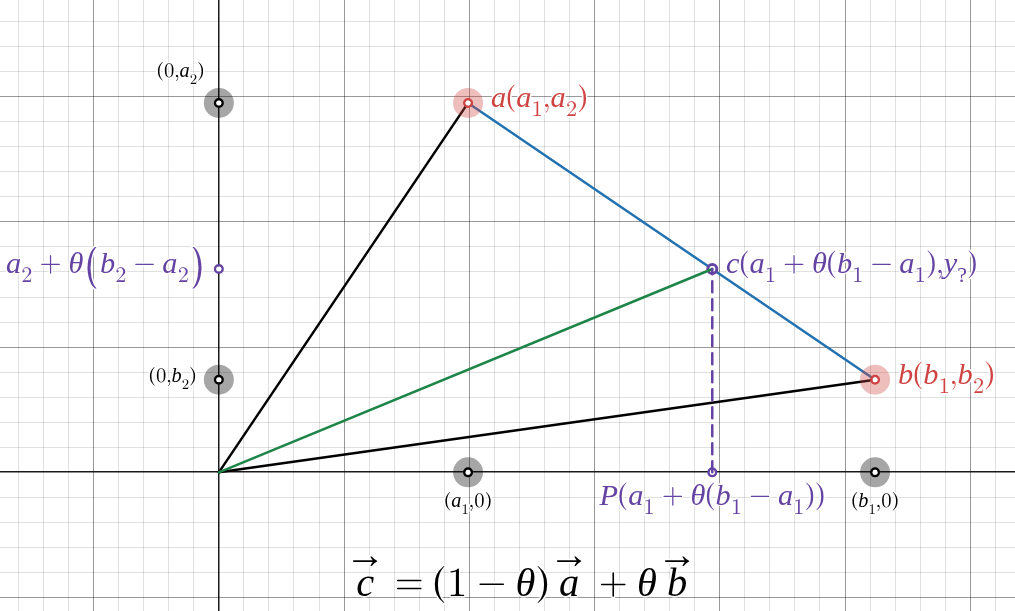
\includegraphics[scale=0.2]{images/affine-combination-2-vecs-2d}
\end{figure}

            We first consider vectors $\boldsymbol{a}=(\boldsymbol{a}_1,\boldsymbol{a}_2),\boldsymbol{b}=(\boldsymbol{b}_1,\boldsymbol{b}_2)$ of size 2.
            By definition, their affine combination, $\boldsymbol{c}$ is a vector: 
            \begin{equation}
            \begin{aligned}
                \boldsymbol{c}&=(1-\theta)\boldsymbol{a}+\theta\boldsymbol{b}\\
                \therefore\boldsymbol{c}&=(1-\theta)(\boldsymbol{a}_1+\boldsymbol{a}_2)+\theta(\boldsymbol{b}_1+\boldsymbol{b}_2)\\
            \end{aligned}
            \end{equation}
                which, after applying properties of vector addition [\ref{ss:vector-addition-properties}] and vector-scalar multiplication [\ref{ss:scalar-vector-multiplication-properties}] (note: symbols like $+,-,\cdot$ (even implicit multiplication which usually carries no symbols) are overloaded: $(1-\theta)$ is the difference of two scalars and is therefore a scalar, whereas $\boldsymbol{b}_1+\boldsymbol{b}_2$ is the sum of two vectors and is therefore a vector), becomes
            \begin{equation}
                \label{eq:aff-comb-c-a-b}
            \begin{aligned}
                \boldsymbol{c}=\boldsymbol{a}_1+\theta(\boldsymbol{b}_1-\boldsymbol{a}_1)+\boldsymbol{a}_2+\theta(\boldsymbol{b}_2-\boldsymbol{a}_2)
            \end{aligned}
            \end{equation}

        Equation [\ref{eq:aff-comb-c-a-b}] implies that the point representing the vector $\boldsymbol{c}$ has two elements (or components) whose magnitudes are $a_1+\theta(b_1-a_1)$ (the `horizontal' component) and $a_2+\theta(b_2-a_2)$ (the `vertical' component) respectively\footnote{We do not use bold symbols to denote magnitudes which are always scalar; the scalar $a_1$ is a much simpler notation for the magnitude or length of the vector $\boldsymbol{a}_1$ than $\lvert\boldsymbol{a}_1\rvert$.}.

        We shall now show that this point lies on the straight line joining $\boldsymbol{ab}$.

        Consider the point $P$ which, for $0\leq\theta\leq 1$, lies between $(a_1,0)$ and $(b_1,0)$. A vertical at $P$ intersects the line $\boldsymbol{ab}$ at $c$. What is the distance $cP$? 

        The slopes of segments $\boldsymbol{ab}$ and $\boldsymbol{ac}$ are the same. Therefore, we can write
            \begin{equation}
                \label{eq:compare-slopes-ab-ac}
            \begin{aligned}
                \frac{y_{\scriptscriptstyle ?}-a_2}{\cancel{a_1}+\theta\bcancel{(b_1-a_1)}-\cancel{a_1}}&=\frac{b_2-a_2}{\bcancel{b_1-a_1}}\\
                \therefore y_{\scriptscriptstyle ?}&=a_2+\theta(b_2-a_2)
            \end{aligned}
            \end{equation}
        From Equations [\ref{eq:aff-comb-c-a-b}] and [\ref{eq:compare-slopes-ab-ac}] we see that $y_{\scriptscriptstyle ?}$ is the same as the vertical component of the affine combination $\boldsymbol{c}$ of the given vectors $\boldsymbol{a,b}$.

        Therefore, $\boldsymbol{c}$ must end at a point on the line joining the given vectors.
        \end{proof}
        \textcolor{red}{\textbf{TBD}}: Extend this to $n$ dimensions\footnote{In higher dimensions, \emph{slope}s are replaced by \emph{direction vector}s or \emph{direction cosine}s (See \cite{slope-higher-dimensions}). The affine combination would then end on the direction vector.}.
\end{reflection}

\section{Inner product}
\begin{definition}[Inner Product of two vectors]
    The standard Inner Product or Dot Product of two $n$-vectors $\boldsymbol{a}=(a_1,a_2,\dots,a_n),\boldsymbol{b}=(b_1,b_2,\dots_,b_n)$ is the scalar $\sum_{i=1}^{n}a_ib_i=a_1a_2+b_1b_2+\dots+a_nb_n$.

    The inner product is denoted as $\boldsymbol{a}^T\boldsymbol{b}$ in this book. The superscript $T$ of the first vector stands for `transpose.' We'll define it later.
\end{definition}

    \begin{equation*}
        \label{eq:inner-product-ex}
    \begin{bmatrix}
        -1\\
        \phantom{-}2\\
        \phantom{-}2
    \end{bmatrix}^T
    \begin{bmatrix}
        \phantom{-}1\\
        \phantom{-}0\\
        -3
    \end{bmatrix}
        =(-1)(1)+(2)(0)+(2)(-3)=-7
    \end{equation*}

\begin{reflection}[What to make of the inner product?]
    How might the inner product have come along? In what way is such `reduction' of two vectors to a scalar interesting? The operations vector addition [\ref{s:vector-addition}] and scalar-vector multiplication [\ref{s:scalar-vector-multiplication}] yield a vector, but the inner product yields a scalar. This means chaining of the inner product is not possible (which precludes \emph{associativity} of this operation on three vectors).

    In a way, this feels like a natural extension of the concept of `multiplication' of two real numbers to vectors. But then why `Inner'? Is there `Outer' too?

    A related thought came to my mind: Should I study Hermann Grassmann's \emph{Creation of Linear Algebra}? 
\end{reflection}

\subsection*{Properties}
\label{ss:properties-inner-product}
\begin{enumerate}
    \item Commutativity. $\boldsymbol{a}^T\boldsymbol{b}=\boldsymbol{b}^T\boldsymbol{a}$.
    \item Associativity with Scalar Multiplication. $(\gamma\boldsymbol{a})^T\boldsymbol{b}=\gamma(\boldsymbol{a}^T\boldsymbol{b})$.
    \item Distributivity with Vector Addition. $\boldsymbol{a}^T(\boldsymbol{b}+\boldsymbol{c})=\boldsymbol{a}^T\boldsymbol{b}+\boldsymbol{a}^T\boldsymbol{c}$.
\end{enumerate}

We can also derive the following from the above:
\begin{itemize}
    \item $\boldsymbol{a}^T(\gamma\boldsymbol{b})=\gamma(\boldsymbol{a}^T\boldsymbol{b})$
    \item $\boldsymbol{a}^T(\boldsymbol{b}+\gamma\boldsymbol{c})=\boldsymbol{a}^T\boldsymbol{b}+\gamma(\boldsymbol{a}^T\boldsymbol{c})$
    \item $(\boldsymbol{a}+\boldsymbol{b})^T(\boldsymbol{c}+\boldsymbol{d})=\boldsymbol{a}^T\boldsymbol{c}+\boldsymbol{a}^T\boldsymbol{d}+\boldsymbol{b}^T\boldsymbol{c}+\boldsymbol{b}^T\boldsymbol{d}$ (In this formula $+$ overloaded: on the LHS it denotes vector addition and on the RHS, scalar addition.)
\end{itemize}

\subsection*{General Examples}
The inner product has some neat properties.
\label{ss:inner-product-ex}
\begin{itemize}
    \item Unit vector. ${\boldsymbol{e}_i}^T\boldsymbol{a}=\boldsymbol{a}_i$.
    \item Sum. $\boldsymbol{1}^T\boldsymbol{a}=\sum_{i=1}^{n}\boldsymbol{a}_i$
    \item Average. $({\boldsymbol{1}/n})^T\boldsymbol{a}=\sum_{i=1}^{n}\boldsymbol{a}_i/n$
    \item Sum of squares. ${\boldsymbol{a}}^T\boldsymbol{a}=\sum_{i=1}^{n}(\boldsymbol{a}_i)^2$
    \item Selective sum. Let $\boldsymbol{b}=(\boldsymbol{b}_i\mid b_i=0\text{ or }1)$. Then $\boldsymbol{a}^T\boldsymbol{b}=\sum_{i=1}^n\boldsymbol{a}_i\quad\forall i\mid\boldsymbol{b}_i=1$.
\end{itemize}

\subsection*{Applications}
\begin{itemize}
    \item Co-occurrence.(This is pretty slick!) 

        We think of each dimension as merely a number. Then, we can think of a subset of those numbers as a Boolean vector!

        If our five numbers or five dimensions are the set\footnote{One issue is that sets have no `order', whereas vectors are essentially ordered. Also, no two dimensions can represent the same number.} $S=\{1,3.4,-3,2.3,20\}$, then its $3$-subset, $T=\{1,-3,2.3\}$, is represented by the vector $\boldsymbol{a}=(1,0,1,1,0)$. A $2$-subset $U=\{3.4,20\}$ is represented by the vector $\boldsymbol{b}=\{0,1,0,0,1\}$. \textbf{The \emph{size}\footnote{To emphasize, it's the size of the set, not the set itself.} of their intersection}, $\mid T\cup U\mid$, is represented by the inner product $\boldsymbol{a}^T\boldsymbol{b}$. In this case, $\boldsymbol{a}^T\boldsymbol{b}=0$; those two sets are disjoint. 

        The size of the intersection is the same as the total number of co-occurrences (common members) of the two sets.

        \begin{reflection}[Creativity is a Harsh Mistress.]
            Isn't that (modeling an $n$-set as an $n$-vector) interesting?

            I appreciate this, I can \emph{see} an $n$-set as an $n$-vector now, but, given sufficient time, would I \emph{think of} such a Boolean-vector model of a mathematical set?
        \end{reflection}
        
    \item Weights, features, and score.
    \item Price-quantity.
    \item Speed-time (total distance).
    \item Probability and expected values.
    \item Polynomial evaluation (polynomial coefficients and integer powers of a value as two $n$-vectors).
    \item Discounted total or net present value (for a given rate of interest).
    \item Portfolio return (vector of fractional returns and vector of portfolio investments).
    \item Document sentiment analysis (crude; categorize every dictionary word using a few sentiment categories and evaluate the sentiment score of documents modeled as histograms of word frequencies).
\end{itemize}

\section{Complexity of vector computations}
\subsection*{Computer representation of numbers (scalars) and vectors}
\subsection*{Floating point operations}
Floating point round-off errors, and methods to mitigate their ill-effect on accuracy of results are studied in \emph{Numerical Analysis}.
\subsection*{Flops and complexity}
\subsection*{Complexity of vector operations}
\subsection*{Complexity of sparse vector operations}

\subsection*{Exercises}
\begin{exercise}
    (1.9) Symptoms vector. A $20$-vector $\boldsymbol{s}$ records whether each of $20$ different symptoms is present in a medical patient, with $\boldsymbol{s}_i=1$ meaning the patient has the symptom and $\boldsymbol{s}_i=0$
meaning she does not. Express the following using vector notation.
\begin{enumerate}[label=(\alph*)]
  \item The total number of symptoms the patient has.
  \item The patient exhibits five out of the first ten symptoms.
\end{enumerate}
\end{exercise}
\textbf{Solution.}
\begin{enumerate}[label=(\alph*)]
        \item Each $1$ in $\boldsymbol{s}$ increments the number of symptoms, each $0$ leaves it unchanged. Therefore, the total number of a patient's symptoms is the sum of $\boldsymbol{s}$ using the ones vector of size $20$: $\boldsymbol{1}^T\boldsymbol{s}$.
    \item The sum of the first $10$ symptoms is of essence. We devise a $20$-vector $\boldsymbol{f}$: 
            \[
                \boldsymbol{f}_i=
               \begin{cases}
                   1,&\text{if $1\leq i\leq 10$}\\
                   0,&\text{otherwise}
               \end{cases}
            \]
         Now, $\boldsymbol{f}^T\boldsymbol{s}$ will count the number of $1$s in the first 10 elements of $\boldsymbol{s}$. It will mask any symptoms numbered $11$ through $20$.
            \[
                \text{Does $\boldsymbol{s}$ exhibit 5 out of the first ten symptoms?}
                \begin{cases}
                    \text{Yes},&\text{if $\boldsymbol{f}^T\boldsymbol{s}\geq 5$}\\
                    \text{No},&\text{otherwise}
                \end{cases}
            \]
    \end{enumerate}
\begin{exercise}
    (1.11) Word count and word count histogram vectors. Suppose an $n$-vector $\boldsymbol{w}$ is the word count vector associated with a document and a dictionary of $n$ words. For simplicity, we will assume that all words in the document appear in the dictionary.
    \begin{enumerate}[label=(\alph*)]
\item What is $\boldsymbol{1}^T\boldsymbol{w}$?
\item What does $\boldsymbol{w}_{\scriptscriptstyle 282}$ mean?
\item Let $\boldsymbol{h}$ be an $n$-vector that gives the histogram of the word counts, i.e., $\boldsymbol{h}_i$ is the fraction of the words in the document that are word $i$. Use vector notation to express $\boldsymbol{h}$ in terms of $\boldsymbol{w}$. (You can assume that the document contains at least one word.)
    \end{enumerate}
\end{exercise}
\textbf{Solution.}
Our dictionary can be thought of as a sequence of $n$ words. It need not be lexically ordered, only indexed by integer. Documents are modeled as $n$-vectors based on how many times each dictionary word appears in them.
\begin{enumerate}[label=(\alph*)]
    \item To construct $\boldsymbol{w}$, the $n$-vector representing the document, we first set all $n$ elements of it to $0$ and start reading the document word-by-word. Upon reading a word, we find its index $i$ in the dictionary (note: we are given that the document does not contain a word not in the dictionary). For example, the first word in the document may be the eighteenth ($i=18$) word in the dictionary. Then, we increment $\boldsymbol{w}_{\scriptscriptstyle i}$ (that is, $\boldsymbol{w}_{\scriptscriptstyle 18}$). Each word increments \emph{some} $\boldsymbol{w}_i$. After we finish reading the document, each $\boldsymbol{w}_i$ equals the number of times $i^{th}$ dictionary word has appeared in the document.
        The inner product
        \[
            \boldsymbol{1}^T\boldsymbol{w}=1\cdot\boldsymbol{w}_1+1\cdot\boldsymbol{w}_2+\dots+1\cdot\boldsymbol{w}_n=\boldsymbol{w}_1+\boldsymbol{w}_2+\dots+\boldsymbol{w}_n
        \]
        This is the word length of the document.

    \item $\boldsymbol{w}_{\scriptscriptstyle 282}$ denotes how many times the $282^{nd}$ dictionary word appears in the document (note: our dictionary is \emph{indexed}).
    \item It follows from the above that $\boldsymbol{h}=(\boldsymbol{h}_i\mid\boldsymbol{h}_i=\frac{\boldsymbol{w}_i}{\boldsymbol{1}^T\boldsymbol{w}}\forall i\;1\leq i\leq n)$
\end{enumerate}


\begin{exercise}
    (1.14) Industry or sector exposure. Consider a set of $n$ assets or stocks that we invest in. Let $\boldsymbol{f}$ be an $n$-vector that encodes whether each asset is in some specific industry or sector, e.g., pharmaceuticals or consumer electronics. Specifically, we take $\boldsymbol{f}_i=1$ if asset $i$ is in the sector, and $\boldsymbol{f}_i=0$ if it is not. 

    Let the $n$-vector $\boldsymbol{h}$ denote a portfolio, with $\boldsymbol{h}_i$ the dollar value held in asset $i$ (with negative meaning a short position\footnote{A financial stance where you \emph{borrow} stock assets and sell them off in the open market almost immediately. You then buy them again so that you can return what you borrowed. In this case, you make a profit only if \emph{the stock price falls before you return}.}). The inner product $\boldsymbol{f}^T\boldsymbol{h}$ is called the (dollar value) exposure of our portfolio to the sector. It gives the net dollar value of the portfolio that is invested in assets from the sector. 

    A portfolio $\boldsymbol{h}$ is called neutral (to a sector or industry) if $\boldsymbol{f}^T\boldsymbol{h}=0$.  A portfolio $\boldsymbol{h}$ is called long-only if each entry is nonnegative, i.e., $\boldsymbol{h}_i\geq 0\;\forall\;i$. This means the portfolio does not include any short positions.

What does it mean if a long-only portfolio is neutral to a sector, say, pharmaceuticals?  Your answer should be in simple English, but you should back up your conclusion with an argument.
\end{exercise}
\textbf{Solution.}

Consider a set of assets: $S=\{t_1, t_2,\dots,t_n\}$, where each $t_i$ represents a stock.
Elements of the $n$-vector $\boldsymbol{f}=(\boldsymbol{f}_1,\boldsymbol{f}_2,\dots,\boldsymbol{f}_n)$ (let's call this vector \emph{sector}) is defined thus:

            \[
                \boldsymbol{f}_i=
               \begin{cases}
                   1,&\text{if $t_i$ is in the sector represented by $\boldsymbol{f}$}\\
                   0,&\text{otherwise}
               \end{cases}
            \]

The $n$-vector that is our \emph{portfolio}, i.e., $\boldsymbol{h}=(\boldsymbol{h}_1,\boldsymbol{h}_2,\dots,\boldsymbol{h}_n)$.

Since our $\boldsymbol{h}$ is \emph{long-only}, $\boldsymbol{h}_i\geq 0\;\forall i$. The trivial case where we have a $\boldsymbol{0}$ portfolio vector is literally ungainly. We therefore assume that there is some $\boldsymbol{h}_i>0$.

For $\boldsymbol{h}$ to be neutral to the sector represented by $\boldsymbol{f}$, 
\begin{equation}
    \label{eq:portfolio-sector-inner-product}
    \begin{aligned}
        \boldsymbol{f}^T\boldsymbol{h}&=0\\
        \therefore\boldsymbol{f}_1\boldsymbol{h}_1+\boldsymbol{f}_2\boldsymbol{h}_2+\dots+\boldsymbol{f}_n\boldsymbol{h}_n&=0
    \end{aligned}
\end{equation}

Since each $\boldsymbol{f}_i$ and $\boldsymbol{h}_i$ are nonnegative and $\sum_{i=1}^{n}\boldsymbol{f}_i\boldsymbol{h}_i$ equals $0$ (i.e., Equation [\ref{eq:portfolio-sector-inner-product}] holds), each $\boldsymbol{f}_i\boldsymbol{h}_i$ must be zero. This will happen when $\boldsymbol{h}_i$ is $0$ when $\boldsymbol{f}_i$ is nonzero. Thus, our long-only portfolio is neutral to a sector when we have not invested in any stocks that belong to that sector.

\textbf{Example.} 

Let $S=\{\text{NVDA,APPL,JNJ,TSLA,META}\}$.

Let's consider the Information Technology (IT) sector in which NVDA and APPL fall (JNJ: Health Care, TSLA: Consumer Discretionary, META: Communication Services). Therefore, $\boldsymbol{f}=(1,1,0,0,0)$.

Therefore, for our long-only portfolio to be neutral to the IT sector (i.e., for $\boldsymbol{f}^T\boldsymbol{h}$ to be $0$), we must have $\boldsymbol{h}_1=\boldsymbol{h}_2=0$.

\begin{reflection}[A Fallacy!]
This is how wrote it at first. Upon thinking more, the fallacy was clear. What was I smoking? Gosh!

{\color{red} {
        For Equation [\ref{eq:portfolio-sector-inner-product}] to hold, with a non-$\boldsymbol{0}$ $\boldsymbol{h}$, either 1) some $\boldsymbol{h}_i$ must be negative, or 2) $\boldsymbol{f}$ must be $\boldsymbol{0}$.

    However, since our portfolio is long-only, no $\boldsymbol{h}_i$ is negative. Therefore, for our portfolio to be neutral with respect to a sector, our sector vector, $\boldsymbol{f}$, must be $\boldsymbol{0}$. We hold no assets of that sector if our portfolio is long-only.
    (That last sentence is even more wrong!)}
}

\end{reflection}

\begin{exercise} (1.15) Cheapest supplier. You must buy $n$ raw materials in quantities given by the $n$-vector $\boldsymbol{q}$, where $\boldsymbol{q}_i$ is the amount of raw material $i$ that you must buy. $K$ potential suppliers offer the raw materials at prices given by the $n$-vectors $p_1,p_2,\dots,p_K$. (Note that $p_k\;1\leq k\leq K$ is an $n$-vector; ${(p_k)}_i$ is the price that supplier $k$ charges per unit of raw material $i$.) We will assume that all quantities and prices are positive.

If you must choose just one supplier, how would you do it? Your answer should use vector notation.

    A (highly paid) consultant tells you that you might do better (i.e., get a better total cost) by splitting your order into two, by choosing two suppliers and ordering $(1/2)\boldsymbol{q}$ (i.e., half the quantities) from each of the two. He argues that having a diversity of suppliers is better. Is he right? 

    If so, explain how to find the two suppliers you would use to fill half the order.
\end{exercise}
\textbf{Solution.}
\[
    \text{Total Cost $T_i$ for the supplier $i$}=\boldsymbol{q}^T\boldsymbol{p}_i=\boldsymbol{q}_1(\boldsymbol{p}_i)_1+\boldsymbol{q}_2(\boldsymbol{p}_i)_2+\dots+\boldsymbol{q}_n(\boldsymbol{p}_i)_n
\]
Thus, the inner product $\boldsymbol{q}^T\boldsymbol{p}_i$ (note: $\boldsymbol{p}_i$ and $\boldsymbol{q}$ are both $n$-vectors) gives the total cost incurred in procuring the raw materials from the supplier $i$.

Calculating the inner product for every vendor gives us total cost of procuring the raw materials for a full order from them. This constructs a (sorted) permutation $\left\langle T_1,T_2,T_3,\dots,T_K\right\rangle\mid T_i\leq T_{i+1}$ of the $K$ numbers. Since `better' means ``incurring least total cost,'' the supplier with total cost $T_1$ should be picked.

The consultant's premise, ``The more diverse the better,'' is alright for diversity, but not necessarily so for the total cost.

Consider two suppliers $i,j$ whose price vectors are $\boldsymbol{p}_i,\boldsymbol{p}_j$ and total costs for the full order $\boldsymbol{q}$ are $T_i=\boldsymbol{q}^T\boldsymbol{p}_i,T_j=\boldsymbol{q}^T\boldsymbol{p}_j$ respectively. Let $T_i\leq T_j$. Let's say that we split our order equally between these two suppliers. Then, the total cost would be $\frac{1}{2}\boldsymbol{q}^T\boldsymbol{p}_i+\frac{1}{2}\boldsymbol{q}^T\boldsymbol{p}_j=\frac{1}{2}(T_i+T_j)\geq\frac{1}{\cancel{2}}(\cancel{2}T_i)$, i.e., total cost $\geq T_i$ (the equality holds only when $T_i=T_j$, that is, when the two suppliers cost us the same.)

If suppliers quoted per-unit prices assuming a full order, would they accept only half an order?

I wonder why the consultant is highly paid!

\begin{exercise}
    (1.16) Inner product of nonnegative vectors. A vector is called nonnegative if all its entries are nonnegative.
\begin{enumerate}[label=(\alph*)]
    \item Explain why the inner product of two nonnegative vectors is nonnegative.
    \item Suppose the inner product of two nonnegative vectors is zero. What can you say about them? Your answer should be in terms of their respective sparsity patterns, i.e., which entries are zero and nonzero.
\end{enumerate}
\end{exercise}
\textbf{Solution.}
Consider two nonnegative $n$-vectors, $\boldsymbol{a,b}$. By definition, $\boldsymbol{a}_i\geq 0,\boldsymbol{b}_i\geq 0\;\forall i\; 1\leq i\leq n$.
\begin{enumerate}[label=(\alph*)]
    \item $\boldsymbol{a}^T\boldsymbol{b}=\sum_{i=1}^{n}\boldsymbol{a}_i\boldsymbol{b}_i$. From the above definition, $0\leq\boldsymbol{a}_i\boldsymbol{b}_i\;\forall i$. It then follows that $0\leq\sum_{i=1}^{n}\boldsymbol{a}_i\boldsymbol{b}_i$, that is, $0\leq\boldsymbol{a}^T\boldsymbol{b}$.
    \item If $\boldsymbol{a}^T\boldsymbol{b}=0$, and $\boldsymbol{a}_i\boldsymbol{b}_i\geq 0\;\forall i$, then $\boldsymbol{a}_i\boldsymbol{b}_i=0\;\forall i$. Thus, $\exists i\mid\boldsymbol{a}_i\ne 0\implies \boldsymbol{b}_i=0$ and vice versa. Thus, if $\nnz{\boldsymbol{a}}=n_1$, then $\nnz{\boldsymbol{b}}$ must be less than or equal to $n-n_1$.
\end{enumerate}

\begin{exercise}
    (1.18) Linear combinations of linear combinations. Suppose that each of the vectors $\boldsymbol{b}_1,\boldsymbol{b}_2,\dots,\boldsymbol{b}_k$ is a linear combination of the vectors $\boldsymbol{a}_1,\boldsymbol{a}_2,\dots,\boldsymbol{a}_m$, and $\boldsymbol{c}$ is a linear combination of $\boldsymbol{b}_1,\boldsymbol{b}_2,\dots,\boldsymbol{b}_k$.  Then $\boldsymbol{c}$ is a linear combination of $\boldsymbol{a}_1,\boldsymbol{a}_2,\dots,\boldsymbol{a}_m$. Show this for the case with $m=k=2$.  (Showing it in general is not much more difficult, but the notation gets more complicated.)

\end{exercise}
\textbf{Solution.}
We define the following for $k=m=2$.
\begin{equation}
    \label{eq:abc-definitions}
    \begin{aligned}
        \boldsymbol{b}_1&=\alpha_{11}\boldsymbol{a}_1+\alpha_{12}\boldsymbol{a}_2\\
        \boldsymbol{b}_2&=\alpha_{21}\boldsymbol{a}_1+\alpha_{22}\boldsymbol{a}_2\\
        \boldsymbol{c}&=\beta_1\boldsymbol{b}_1+\beta_2\boldsymbol{b}_2
    \end{aligned}
\end{equation}

Then, it follows that $\boldsymbol{c}=(\beta_1\alpha_{11}+\beta_2\alpha_{21})\boldsymbol{a}_1+(\beta_1\alpha_{12}+\beta_2\alpha_{22})\boldsymbol{a}_2\implies\boldsymbol{c}=\gamma_1\boldsymbol{a}_1+\gamma_2\boldsymbol{a}_2$ (since parenthesized terms are scalars). Therefore, linear combination of a linear combination is a linear combination.

\begin{exercise}
    (1.19) Auto-regressive model. Suppose that $z_1,z_2,\dots$ is a time series, with the number $z_t$ giving the value in period or time $t$. For example, $z_t$ could be the gross sales at a particular store on day $t$. An auto-regressive (AR) model is used to predict $z_{t+1}$ from the previous $M$ values, $z_{\scriptscriptstyle t},z_{\scriptscriptstyle t-1},\dots,z_{\scriptscriptstyle t-M+1}$:
    \begin{equation}
        \label{eq:ar-model}
        \hat{z}_{\scriptscriptstyle t+1} = (z_{\scriptscriptstyle t},z_{\scriptscriptstyle t-1},\dots,z_{\scriptscriptstyle t-M+1})^T\boldsymbol{\beta},\quad t=M,M+1,\dots
    \end{equation}
    Here, $\hat{z}_{\scriptscriptstyle t+1}$ is the model's \underline{prediction} of $z_{\scriptscriptstyle t+1}$, $M$ is the \underline{memory length} of the AR model, and the $M$-vector $\boldsymbol{\beta}$ is the AR model's \underline{coefficient vector}.

    For this problem, we will assume that the time period is daily, and $M=10$. Thus, this AR model predicts tomorrow's value, given the values for the last 10 days.

    For each of the following cases, give a short interpretation or description of the AR model in English, without referring to mathematical concepts like vectors, inner product, and so on. You can use words like `yesterday' or `today'.

\begin{enumerate}[label=(\alph*)]
    \item $\boldsymbol\beta=\boldsymbol{e}_1$ (i.e., the unit $M$-vector with first element $1$ and all other zero.) (I don't understand why the book uses `$\approx$' (i.e., \verb|\approx| here instead of `$=$').
    \item $\boldsymbol\beta=2\boldsymbol{e}_1-\boldsymbol{e}_2$.
    \item $\boldsymbol\beta=\boldsymbol{e}_6$.
    \item $\boldsymbol\beta=0.5\boldsymbol{e}_1+0.5\boldsymbol{e}_2$.
\end{enumerate}
\end{exercise}
\textbf{Solution.}
The essence of the AR model is in the coefficient vector, $\boldsymbol\beta$, for the given $M$.

\begin{enumerate}[label=(\alph*)]
    \item From Equation [\ref{eq:ar-model}], if $\boldsymbol\beta=(1,0,0,\dots,0)$, then 
        \begin{equation*}
            \begin{aligned}
                \hat{z}_{\scriptscriptstyle t+1}&=\boldsymbol{z}^T\boldsymbol\beta\\
                                                &=\boldsymbol{z}_{\scriptscriptstyle t}\cdot 1+\boldsymbol{z}_{\scriptscriptstyle t-1}\cdot 0+\dots+\boldsymbol{z}_{\scriptscriptstyle t-M+1}\cdot 0\\
                                                &=\boldsymbol{z}_t
            \end{aligned}
        \end{equation*}

        In this case, the AR model predicts that the amount of gross sales tomorrow will be the same as the amount today\footnote{This reminds me of a weather forecast joke: The meteorological department always predicts rainy tomorrow if it rained today; that way, they have a $50\%$ chance of being accurate, but more people believe the department's forecasts.}.
    \item From Equation [\ref{eq:ar-model}], if $\boldsymbol\beta=2\boldsymbol{e}_1-\boldsymbol{e}_2=(2,-1  ,0,\dots,0)$, then 
        \begin{equation*}
            \begin{aligned}
                \hat{z}_{\scriptscriptstyle t+1}&=\boldsymbol{z}^T\boldsymbol\beta\\
                                                &=\boldsymbol{z}_{\scriptscriptstyle t}\cdot 2-\boldsymbol{z}_{\scriptscriptstyle t-1}\cdot 1+0+0+\dots+\boldsymbol{z}_{\scriptscriptstyle t-M+1}\cdot 0\\
                                                &=2\boldsymbol{z}_t-\boldsymbol{z}_{\scriptscriptstyle t-1}
            \end{aligned}
        \end{equation*}
        The sales tomorrow are expected to be double that of today less that of yesterday.
    \item Along the similar lines, the sales tomorrow are expected to be the same as that of 6 days ago.
    \item Along the similar lines, the sales tomorrow are expected to be half of today plus half of yesterday.
\end{enumerate}
\begin{exercise}
    (1.20) How many bytes does it take to store $100$ vectors of length $10^5$? How many flops does it take to form a linear combination of them (with $100$ nonzero coefficients)? About how long would this take on a computer capable of carrying out $1$ Gflop/s?
\end{exercise}
\textbf{Solution.}
\begin{enumerate}[label=(\alph*)]
    \item The vector with $10^5$ real numbers takes up $800,000$ bytes, $100$ such vectors $80,000,000$ bytes, or $80$ Megabytes.
    \item There are $10^5$ multiplications (flops) per vector, so $10^7$ flops for 100 vectors, producing 100 numbers which we sum. That is $99$ flops more. All told, that is $10,000,099$ flops.
    \item A $1$ Gflop/s computer may take a little more than $\frac{1.0000099\times 10^7}{10^9}$ s, that is, a little over $10$ milliseconds.
\end{enumerate}

\chapter{Linear Functions}

In this chapter  we introduce linear and affine functions, and describe some common settings where they arise, including \emph{regression models}.

\section{Linear functions}

\subsection*{Function notation.}
The notation $f:\mathbb{R}^n\rightarrow\mathbb{R}$ means that $f$ is a function that maps real $n$-vectors to real numbers, i.e., it is a scalar-valued function of $n$-vectors.

If $\boldsymbol{x}$ is an $n$-vector, then $f(\boldsymbol{x})$, which is a scalar, denotes the value of the function $f$ at $\boldsymbol{x}$. (In the notation $f(x)$, $x$ is referred to as the \emph{argument} of the function.)

We can also interpret $f$ as a function of $n$ scalar arguments, the entries of the vector argument, in which case we write $f(\boldsymbol{x})$ as $f(\boldsymbol{x}) = f(\boldsymbol{x}_1, \boldsymbol{x}_2,\dots,\boldsymbol{x}_n)$.

Here we refer to $x_1,x_2,\dots,x_n$ as the \emph{argument\underline{s}} of $f$. 

We sometimes say that $f$ is real-valued, or scalar-valued, to emphasize that $f(\boldsymbol{x})$ is a real number or scalar (although clearly its argument isn't a real number).

\textbf{Example.} $f:\mathbb{R}^4\rightarrow\mathbb{R}\;f(\boldsymbol{x})=\boldsymbol{x}_1+\boldsymbol{x}_2-\boldsymbol{x}_4^2$.

\subsection*{Inner product function.}
Suppose $\boldsymbol{a}$ is an $n$-vector. We can define a real-valued function $f:\mathbb{R}^n\rightarrow\mathbb{R}$ given by: 
\begin{equation}
    \label{eq:inner-product-function}
    f(\boldsymbol{x})=\boldsymbol{a}^T\boldsymbol{x}=\boldsymbol{a}_1\boldsymbol{x}_1+\boldsymbol{a}_2\boldsymbol{x}_2+\dots+\boldsymbol{a}_n\boldsymbol{x}_n
\end{equation}
We can also think of $f$ as forming a weighted sum of the elements of $\boldsymbol{x}$; the elements of $\boldsymbol{a}$ give the weights used in forming it.
\subsection*{Superposition and linearity.}
The inner product function (Equation [\ref{eq:inner-product-function}]) satisfies a rather peculiar property:
\begin{equation}
    \label{eq:superposition}
    \begin{aligned}
        f(\alpha\boldsymbol{x}+\beta\boldsymbol{y})&=\boldsymbol{a}^T(\alpha\boldsymbol{x}+\beta\boldsymbol{y})\\
                                                   &=\alpha\boldsymbol{a}^T\boldsymbol{x}+\beta\boldsymbol{a}^T\boldsymbol{y}\\
                                                   &=\alpha f(\boldsymbol{x})+\beta f(\boldsymbol{y})\\
                                                   \text{$\forall\;n$-vectors $\boldsymbol{x,y}$, and scalars $\alpha,\beta$}
    \end{aligned}
\end{equation}
This property is called \emph{superposition}. 

\begin{definition}[Linear Function]
    \label{def:linear-function}
A function $f:\mathbb{R}^n\rightarrow\mathbb{R}$ that satisfies the superposition property is called a \emph{linear function}.
\end{definition}

\begin{reflection}[Alternate form of Equation [\ref{eq:superposition}]
    I slightly rearranged Equation [\ref{eq:superposition}]. This rearrangement makes its form a little more consistent with its name (of course, in my opinion).
\begin{equation}
    \label{eq:superposition-alternate-form}
    \begin{aligned}
        f(\alpha\boldsymbol{x}+\beta\boldsymbol{y})&=\boldsymbol{a}^T(\alpha\boldsymbol{x}+\beta\boldsymbol{y})\\
                                                   &=\boldsymbol{a}^T(\alpha\boldsymbol{x})+\boldsymbol{a}^T(\beta\boldsymbol{y})\\
        \therefore f(\alpha\boldsymbol{x}+\beta\boldsymbol{y})&=f(\alpha\boldsymbol{x})+f(\beta\boldsymbol{y})\\
                                                   \text{$\forall\;n$-vectors $\boldsymbol{x,y}$, and scalars $\alpha,\beta$}
    \end{aligned}
\end{equation}
    Equation [\ref{eq:superposition-alternate-form}] tells us that a function $f:\mathbb{R}^n\rightarrow\mathbb{R}$ is linear if applying it to a linear combination of $n$-vectors is equivalent to combining (by addition or subtraction) the results of applying it to the elements of the linear combination (hence \emph{superposition} or \emph{superimposition}, that is, overlaying, placing on top of).
\end{reflection}

If a function $f$ is linear, superposition extends to linear combinations of any finite number of vectors.

We can break the superposition property (Equation [\ref{eq:superposition}]) into two properties as applicable to $f:\mathbb{R}^n\rightarrow\mathbb{R}$:
\begin{enumerate}
    \item Homogeneity: $f(\alpha\boldsymbol{x})=\alpha f(\boldsymbol{x})$. Applying $f$ to a scaled vector is equivalent to scaling the result of applying $f$ to it. 
    \item Additivity: $f(\boldsymbol{x}+\boldsymbol{y})=f(\boldsymbol{x})+f(\boldsymbol{y})$. Applying $f$ to the sum of two vectors is equivalent to the sum of the results of its application to the individual vectors.
\end{enumerate}

\subsection*{Inner product representation of a linear function.}
We saw that the inner product function is linear. 

The converse is also true.

A linear function can be expressed as an inner product of its argument ($n$-vector) with some fixed $n$-vector.

The observation is remarkable and its proof elegant!

\begin{theorem}[Linearity $\implies$ Existence of inner product]
    \label{th:linearity->inner-product}
    If $f:\mathbb{R}^n\rightarrow\mathbb{R}$ is linear (when applied to an $n$-vector $\boldsymbol{x}$), then there exists a vector $\boldsymbol{a}$, such that $f(\boldsymbol{x})=\boldsymbol{a}^T\boldsymbol{x}$.
\end{theorem}
\begin{proof}
    Let $\boldsymbol{x}=(\boldsymbol{x}_1,\boldsymbol{x}_2,\dots,\boldsymbol{x}_n)$.
    Then,
    \begin{align*}
        \label{eq:Th 2.1}
            \boldsymbol{x}&=\boldsymbol{x}_1\boldsymbol{e}_1+\boldsymbol{x}_2\boldsymbol{e}_2+\dots+\boldsymbol{x}_n\boldsymbol{e}_n\\
            &\text{where each $\boldsymbol{x}_i$ is a scalar, and $\boldsymbol{e}_i$ is the $i^{\scriptscriptstyle th}$ unit $n$-vector}\\
            \therefore f(\boldsymbol{x})&=f(\boldsymbol{x}_1\boldsymbol{e}_1+\boldsymbol{x}_2\boldsymbol{e}_2+\dots+\boldsymbol{x}_n\boldsymbol{e}_n)\\
            &\text{$f$ \emph{is} linear, therefore, it satisfies the superposition property for $n$ vectors:}\\
            f(\boldsymbol{x})&=\boldsymbol{x}_1f(\boldsymbol{e}_1)+\boldsymbol{x}_2f(\boldsymbol{e}_2)+\dots+\boldsymbol{x}_nf(\boldsymbol{e}_n)\\
                &=(f(\boldsymbol{e}_1),f(\boldsymbol{e}_2),\dots,f(\boldsymbol{e}_n))^T(\boldsymbol{x}_1,\boldsymbol{x}_2,\dots,\boldsymbol{x}_n) \tag{Th 2.1}\\
                &=\boldsymbol{a}^T\boldsymbol{x}\\
                &\text{where $\boldsymbol{a}=(f(\boldsymbol{e}_1),f(\boldsymbol{e}_2),\dots,f(\boldsymbol{e}_n))$} 
    \end{align*}
\end{proof}

\begin{reflection}[A Remarkable Observation]
    This is neat! If a real-valued function ($f:\mathbb{R}^n\rightarrow\mathbb{R}$) applied to a vector argument $\boldsymbol{x}$ is linear, then $f(x)=(f(\boldsymbol{e}_1),f(\boldsymbol{e}_2),\dots,f(\boldsymbol{e}_n))^T\boldsymbol{x}$.
\end{reflection}


The formula [\ref{eq:Th 2.1}] has interesting implications:
\begin{itemize}
    \item Consider a \emph{linear} $f:\mathbb{R}^n\rightarrow\mathbb{R}$. To predict or calculate $f(\boldsymbol{x})$ (an arbitrary vector) whose elements $\boldsymbol{x}_1,\boldsymbol{x}_2,\dots,\boldsymbol{x}_n$ we know, we compute or observe $f$'s value (response) on $n$ vectors, $\boldsymbol{e}_1,\boldsymbol{e}_2,\dots,\boldsymbol{e}_n$ (note: these are $n$ unit $n$-vectors) and then take the inner product of those $n$ values with $n$ elements of $\boldsymbol{x}$.  
    \item The vector $\boldsymbol{a}=(f(\boldsymbol{e}_1),f(\boldsymbol{e}_2),\dots,f(\boldsymbol{e}_n))$ is \emph{unique}.
\end{itemize}

\subsection*{Examples}
\label{ss:linear-function-examples}
\begin{itemize}
    \item The \emph{Average} function. $\text{avg}({\boldsymbol{x}})=\bar{\boldsymbol{x}}=\frac{1}{n}\sum_{i=1}^{n}\boldsymbol{x}_i$. Linear.
    \item The \emph{Maximum} (or \emph{Minimum}) function. $\max(\boldsymbol{x})=\max(\boldsymbol{x}_i\mid 1\leq i\leq n)$. Not linear. See problem [\ref{pr:max-func-not-affine}] later.
\end{itemize}

\begin{reflection}[Is discovering mathematics inexplicable?]
    I am quite excited about this link between linearity of $f$ and existence of an inner product vector, $\boldsymbol{a}=(f(\boldsymbol{e}_1),f(\boldsymbol{e}_2),\dots,f(\boldsymbol{e}_n))$. It feels like a magical discovery. 

    Can I think of another linear function? What examples, other than the sort of obvious $\text{avg}(\boldsymbol{x})$ and $\max(\boldsymbol{x})$, are there?

    Yes, I know the definition: If $f(\alpha\boldsymbol{x}+\beta\boldsymbol{y})=\alpha f(\boldsymbol{x})+\beta f(\boldsymbol{y})$, then $f$ is linear. However, is there a deeper insight that lets me find such functions more easily?

    I rummage through the standard single-variable functions (polynomial, rational, trigonometric, exponential, logarithmic). That doesn't help. Should the statistical functions (that operate on several numbers) like \texttt{avg} be considered?
\end{reflection}


\subsection*{Affine functions.}
(See also: Affine combination, subsection [\ref{ss:special-linear-combinations}])
\begin{definition}[Affine Function]
    \label{def:affine-function}
    A linear function $f:\mathbb{R}^n\rightarrow\mathbb{R}$ (See definition [\ref{def:linear-function}]) is affine \emph{if and only if} it can be expressed as $f(\boldsymbol{x})=\boldsymbol{a}^T\boldsymbol{x}+b$ for some $n$-vector $\boldsymbol{a}$ and scalar $b$ (sometimes called \emph{offset}).
\end{definition}

For example, the function on $3$-vectors defined by $f(\boldsymbol{x})=2.3−2\boldsymbol{x}_1+1.3\boldsymbol{x}_2−\boldsymbol{x}_3$, is affine, with $b=2.3,\boldsymbol{a}=(−2, 1.3, −1)$.

\begin{reflection}[Doubts on the above definition (\ref{def:affine-function})]
    Some doubts:
    \begin{itemize}
        \item Is $f$ an affine function if $b=0$? I guess not. It seems that given $f(\boldsymbol{x})=\boldsymbol{a}^T+b$, if $b=0$, it's linear, otherwise affine (of course, the superposition property must hold).
    \end{itemize}
\end{reflection}

\begin{theorem}[The Restricted Superposition Property]
    \label{th:affine-function-superposition}
    Any affine function (See definition [\ref{def:affine-function}]) satisfies the superposition property (See equation [\ref{eq:superposition}]) so that $\alpha+\beta=1$.
\end{theorem}
\begin{proof}
    \begin{reflection}
        I proved it on paper. Typesetting it here now.
    \end{reflection}

    $f:\mathbb{R}^n\rightarrow\mathbb{R}$ is an affine function. 
    \begin{equation}
        \label{eq:affine-function-superposition-1}
        f(\boldsymbol{x})=\boldsymbol{a}^T\boldsymbol{x}+b
    \end{equation}

    This means it is linear and satisfies the superposition property (equation [\ref{eq:superposition}]):
    \begin{equation}
        \label{eq:affine-function-superposition-2}
        \begin{aligned}
            f(\alpha\boldsymbol{x}+\beta\boldsymbol{y})&=\alpha f(\boldsymbol{x})+\beta f(\boldsymbol{y})\\
            \therefore\boldsymbol{a}^T(\alpha\boldsymbol{x}+\beta\boldsymbol{y})+b&=\alpha(\boldsymbol{a}^T\boldsymbol{x}+b)+\beta(\boldsymbol{a}^T\boldsymbol{y}+b)\\
            \text{simplifying after }&\text{canceling the vectors on both sides},\\
            \cancel{b}&=\cancel{b}(\alpha+\beta)\quad\quad(\text{We assume that } b\ne 0)\\
            \therefore\alpha+\beta&=1
        \end{aligned}
    \end{equation}
\end{proof}

\begin{reflection}[Logical foundations of mathematics]
    The book argues that the above theorem ([\ref{th:affine-function-superposition}]) can be used to show that a given function is \emph{\underline{not}} affine. And I am not convinced. It all boils down to good definitions and logic, in particular, to material implication ($\mathcal{S}\implies\mathcal{N}$) and material equivalence ($\mathcal{P}\iff\mathcal{Q}$).

    \textbf{I am assuming that for a linear function to be affine, the offset, $b$ must be nonzero}. I wish the book had stated that. From my proof above (Theorem [\ref{th:affine-function-superposition}]), it is clear that for $\alpha+\beta$ to equal $1$, $b$ may not be $0$. 

    It then follows that if some $f:\mathbb{R}^n\rightarrow\mathbb{R}$ (applied to an argument $\boldsymbol{x}$) can only be expressed as $\boldsymbol{a}^T\boldsymbol{x}$, then it is linear, but not affine (because $b$ equals $0$).

    My recipe to show that some $f:\mathbb{R}^n\rightarrow\mathbb{R}$ is affine is simple:
    \begin{enumerate}
        \item Show that $f$ is linear (that is, it satisfies the superposition property), \emph{and}
        \item Show that $\exists\boldsymbol{a}\mid f(\boldsymbol{x})=\boldsymbol{a}^T\boldsymbol{x}+b\;(b\boldsymbol{\ne 0})$.
    \end{enumerate}

    If either of the above is false, $f$ is \emph{not affine}.

    I quote the following (which I like) from the book:

    \epigraph[source=VMLS \cite{bv-app-lin-alg} pp. 31-32]{
        For linear functions, superposition holds for any coefficients $\alpha,\beta,\dots,\omega$; for affine functions, it holds when
    the coefficients sum to $1$ (i.e., when the argument vector, $\boldsymbol{x}$, is an affine combination (See Table [\ref{tab:spl-lin-comb}])).
    }

    That dictates their recipe to show that $f$ is \emph{not affine}: Find a counterexample where $\alpha+\beta=1$ (illustrating with two $n$-vectors) and show that the superposition does not hold (i.e., $f$ is \emph{not linear}) in that case.

    They show that the $\max$ function (See subsection [\ref{ss:linear-function-examples}]) is not affine thus:

    We verified above that superposition does not hold for the $\max$ function (with $n>1$); the coefficients in our counterexample are $\alpha=\beta=\frac{1}{2}$, which sum to one, which allows us to conclude that the $\max$ function is \emph{not affine}.

    How would I show that $\max$ is not affine? I would resort to showing that $\max$ is not linear in general:
    \begin{problem}[The function $\max(\boldsymbol{x})$]
        \label{pr:max-func-not-affine}
        Show that $\max(\boldsymbol{x})$, which results in choosing the value of the biggest element of its argument is not affine.
    \end{problem}
    \begin{proof}
        Let $\boldsymbol{x}=(\boldsymbol{x}_1,\boldsymbol{x}_2,\dots,\boldsymbol{x}_i,\dots,\boldsymbol{x}_n)$.

        Let $\max(\boldsymbol{x})=\boldsymbol{x}_i$. Therefore, $\max(\alpha\boldsymbol{x})=\alpha\boldsymbol{x}_i$.

        Let $\boldsymbol{y}=(\boldsymbol{y}_1,\boldsymbol{y}_2,\dots,\boldsymbol{y}_j,\dots,\boldsymbol{y}_n)$.

        Let $\max(\boldsymbol{y})=\boldsymbol{y}_j$. Therefore, $\max(\beta\boldsymbol{y})=\beta\boldsymbol{y}_j$.

        Then,
        \begin{equation}
            \label{eq:max-func-not-affine-1}
            \max(\alpha\boldsymbol{x})+\max(\beta\boldsymbol{y})=\alpha\boldsymbol{x}_i+\beta\boldsymbol{y}_j
        \end{equation}

        The vector: 

        \begin{equation}
            \label{eq:max-func-not-affine-2}
            \begin{aligned}
                \alpha\boldsymbol{x}+\beta\boldsymbol{y}\\
                &=(\alpha\boldsymbol{x}_1+\beta\boldsymbol{y}_1,\alpha\boldsymbol{x}_2+\beta\boldsymbol{y}_2,\dots,\alpha\boldsymbol{x}_i+\beta\boldsymbol{y}_i,\dots,\alpha\boldsymbol{x}_j+\beta\boldsymbol{y}_j,\dots,\alpha\boldsymbol{x}_n+\beta\boldsymbol{y}_n)
            \end{aligned}
        \end{equation}

        Therefore, $\max(\alpha\boldsymbol{x}+\beta\boldsymbol{y})$ must be one of $\alpha\boldsymbol{x}_i+\beta\boldsymbol{y}_i\;\forall i\;1\leq i\leq n$

        In the general case, then, $\max(\alpha\boldsymbol{x}+\beta\boldsymbol{y})\ne\alpha\boldsymbol{x}_i+\beta\boldsymbol{y}_j$.

        Therefore, $\max$ is not linear and not affine.

    \end{proof}


\end{reflection}


\begin{reflection}[One more on material implication]
    This section has become longer than we need. I, respectfully but rather audaciously, suggest that the authors rewrite it. Although doing so is not standard, they want to differentiate between linear functions (real-valued functions applied to vectors that satisfy superposition, $f=\boldsymbol{a}^T\boldsymbol{x}$) from affine functions (linear functions, $f=\boldsymbol{a}^T\boldsymbol{x}+b, b\ne 0$). They should have more succinctly expressed this intent.

        Linearity (satisfying the superposition property) is a must for any linear and hence affine function. It is \emph{not} that any function that can be expressed as $f=\boldsymbol{a}^T\boldsymbol{x}+b, b\ne 0$ is affine. 

\begin{comment}

    I am commenting this out because it is incorrect. However, I wanted to also document the blind alleys that I run into while studying mathematics \dots

        Here is a \textbf{bogus proof that shows $\max$ is affine}. It commits the \emph{logical fallacy of affirming the consequent of a material implication}: 
        \begin{equation*}
            \begin{split}
                &\mathcal{S}\implies\mathcal{N}\\
                &\mathcal{N}\\
                \hline
                \therefore\;&\mathcal{S}
            \end{split}
        \end{equation*}
        \begin{proof}
            \renewcommand{\qedsymbol}{$\color{red}{\blacksquare}$}
            Consider the function $\max:\mathcal{R}^n\rightarrow\mathcal{R}$ which returns the maximum element of its (vector) argument.

            We'll illustrate with a $4$-vector, but the argument can be generalized to $n$-vectors.

            Let $\boldsymbol{x}=(1,-3,2,-2)$.

            Let $\boldsymbol{a}=(1,1,1,1)$ and $b=4$.
            
            By definition, $\max(\boldsymbol{x})$ is $2$. 

            $\boldsymbol{a}^T\boldsymbol{x}+b=1\cdot 1+1\cdot -3+1\cdot 2+1\cdot -2+4=1-3+2-2+4=2$.

            Since $\boldsymbol{a}^T\boldsymbol{x}+b=\max(\boldsymbol{x})$, $\max$ is affine.

    \end{proof}
\end{comment}
\end{reflection}


\begin{reflection}[That feeling of apprehension ...]

    Linear functions and affine functions were still unclear. I felt uncomfortable. Then, beginning with definitions, I first wrote down implications (I was still unsure about them) and proved them. Then I typeset them below. 
    
    Let's start with definitions. The functions we consider are of type $f:\mathcal{R}^n\rightarrow\mathcal{R}$. The arguments (which are $n$-vectors) to these functions are always written in bold symbols: $\boldsymbol{x},\boldsymbol{y},\boldsymbol{a},\dots$. Scalars are always written with normal emphasis: $b,\alpha,\beta,\dots$. Symbols such as $+$ are context-sensitive: $\boldsymbol{x}+\boldsymbol{y}$, where the arguments are $n$-vectors, is a vector addition that results in an $n$-vector, $a+b$, where the arguments are scalars, is a scalar addition that results in a scalar.
    \begin{definition}[Superposition property (again)]
        \label{def:superposition-property-again}
        $f(\alpha\boldsymbol{x}+\beta\boldsymbol{y})=\alpha f(\boldsymbol{x})+\beta f(\boldsymbol{y})$
    \end{definition}
    \begin{definition}[Restricted superposition property (again)]
        \label{def:restricted-superposition-property-again}
        $f(\alpha\boldsymbol{x}+\beta\boldsymbol{y})=\alpha f(\boldsymbol{x})+\beta f(\boldsymbol{y})\mid\alpha+\beta=1$
    \end{definition}
    \begin{definition}[Linear function (again)]
        $f$ is linear if it satisfies the superposition property. 
    \end{definition}
    \begin{definition}[Affine function (again)]
        $f$ is affine if it satisfies the restricted superposition property. 
    \end{definition}

    \begin{theorem}(Linearity implies inner product)
        \label{th:linearity->inner-product-again}

        If $f$ is linear, then $f(\boldsymbol{x})=\boldsymbol{a}^T\boldsymbol{x}$.
    \end{theorem}
    \begin{proof}
        See Theorem [\ref{th:linearity->inner-product}].
    \end{proof}
    \begin{theorem}(Inner product implies linearity)
        \label{th:inner-product->linearity}
        (This is the converse of the above theorem (Theorem [\ref{th:linearity->inner-product-again}])).

        If $f(\boldsymbol{x})=\boldsymbol{a}^T\boldsymbol{x}$, then $f$ is linear.
    \end{theorem}
    \begin{proof}
        We use properties of vector addition and scalar-vector multiplication and show that the superposition property (See definition [\ref{def:superposition-property-again}]) holds.

        Given, for two $n$-vectors $\boldsymbol{x,y}$: 
        \begin{equation}
            \begin{aligned}
                f(\boldsymbol{x})&=\boldsymbol{a}^T\boldsymbol{x}, f(\boldsymbol{y})=\boldsymbol{a}^T\boldsymbol{y}\\
                \therefore f(\alpha\boldsymbol{x})&=\boldsymbol{a}^T(\alpha\boldsymbol{x})=\alpha\boldsymbol{a}^T\boldsymbol{x}\\
                \therefore f(\beta\boldsymbol{y})&=\boldsymbol{a}^T(\beta\boldsymbol{y})=\beta\boldsymbol{a}^T\boldsymbol{y}\\
                \therefore f(\alpha\boldsymbol{x})+f(\beta\boldsymbol{y})&=\alpha\boldsymbol{a}^T\boldsymbol{x}+\beta\boldsymbol{a}^T\boldsymbol{y}\\
                \therefore f(\alpha\boldsymbol{x})+f(\beta\boldsymbol{y})&=\alpha f(\boldsymbol{x})+\beta f(\boldsymbol{y})\\
                \therefore\text{ $f$ satisfies the}&\text{ superposition property, and is linear.}
            \end{aligned}
        \end{equation}
    \end{proof}
    \begin{theorem}(Affinity implies a special inner product)
        \label{th:affinity->special-inner-product}

        If $f$ is affine, then $f(\boldsymbol{x})=\boldsymbol{a}^T\boldsymbol{x}+b\mid b\ne 0$.

    \end{theorem}
    \begin{proof}
        We use the definition of affine functions, properties of vector addition and scalar-vector multiplication and arrive at a special inner product when we apply $f$ to an arbitrary $n$-vector.
        \begin{reflection}[Reflection inside another Reflection]
            I thought that I nailed these implications, but proving them succinctly is still a challenge. For instance, I have spent quite some time on this confusion: If $f$ is linear (and every affine function is linear), we already know that $f(\boldsymbol{x})=\boldsymbol{a}^T\boldsymbol{x}$. Then, how do you accommodate the additional $b$ when the restricted superposition property ($\alpha+\beta+\dots+\omega=1$) is satisfied? Perhaps we'll need to somehow split $\boldsymbol{a}^T\boldsymbol{x}$ enabled by the fact that the sum of the coefficients is $1$?

            Then, I drew this picture on paper:
            \begin{figure}[H]
                \caption{One way to think about the fine line between affine and linear functions}
                \label{fig:affine-vs-linear}
                \begin{tikzpicture}[
                        binary tree layout,
                        level distance=3cm,
                        sibling distance=5cm,
                    ]
                    \node { 
                        $f(\boldsymbol{x})=\boldsymbol{a}^T\boldsymbol{x}+b$
                    }
                    child {
                        node {
                            $\text{if }\alpha+\beta\ne 1\text{ then }b=0$
                        }
                        edge from parent 
                        node[midway, left, red] {linear}
                    }
                    child {
                        node {
                            $\text{else (that is, }\alpha+\beta=1\text{) }b\ne 0$
                        }
                        edge from parent 
                        node[midway, right, red] {affine}
                    };
                \end{tikzpicture}
            \end{figure}
        \end{reflection}
            \textcolor{red}{\textbf{TBD: Revisit}}
    \end{proof}
    \begin{theorem}(A special inner product implies affinity)
        \label{th:special-inner-product->affinity}
        (This is the converse of the above theorem (Theorem [\ref{th:affinity->special-inner-product}])).

        If $f(\boldsymbol{x})=\boldsymbol{a}^T\boldsymbol{x}+b\mid b\ne 0$, then $f$ is affine.
    \end{theorem}
    \begin{proof}
            \textcolor{red}{\textbf{TBD: Revisit}}
    \end{proof}
\end{reflection}

\subsection*{A civil engineering example.} 

Many scalar-valued functions that arise in science and engineering are well approximated by linear or affine functions.







\printbibliography
\end{document}
